\section{Resampling Study}

To test the ecological validity of findings in experiment 1 and 2 we have also designed a
resampling study based on European Values Survey data.
Variables in the EVS data are not generated artificially from continuous normal distributions 
but are discrete numerical items that are only treated as such by researchers.
By using data gathered for an actual survey, we can observe whether the relative 
performances of the imputation methods change when they are deployed for real data research.

The resampling study follows a similar strategy to that used in the simulations. 
To assess the statistical validity of the different imputation methods we have repeated the 
following steps 500 times ($R = 500$):

\begin{enumerate}
	\item Data generation - A bootstrap sample $\bm{X}^{*}$ is generated by sampling with replacement $n$ 
		observations from a pre-processed EVS data-matrix. 
		Part of the pre-processing step is some form of imputation used to obtain a pseudo-fully observed 
		input data matrix so that $\bm{X}^{*}$ is fully observed;
	\item Missing data imposition - Missing values are imposed on a given number of target variables
		in $\bm{X}^{*}$, according to some response model (see below), and $\bm{X}^{*}_{miss}$ is 
		obtained;
	\item Imputations - Each method described in section 2 is used to deal with missing values
		in $\bm{X}^{*}_{miss}$.
	\item Analysis - Two analysis models are fitted to the differently treated data.
		Parameters estimates are pooled across the differently imputed datasets, for the MI methods, and
		stored along with the estimates obtained with single imputation methods and complete case 
		analysis.
\end{enumerate}

	The average estimate, over the $R$ repetitions, obtained with the Gold Standard approach are considered 
	as ``true" reference values of the parameters in the analysis models.
	The $R$ estimates obtained with all other methods are used to obtain performance measures for each imputation 
	method using the same criteria described for study 1 and 2 (see \ref{criteria}).

	The code to run the simulation was written in the R statistical programming language (version 4.0.3). 
	The resampling study was run using a 2.6 GHz Intel Xeon(R) Gold 6126 processor, 523780 MB of Memory. The
	operating system was Windows Server 2012 R2.

	Computations were run in parallel across the available cores (between 30). Parallel computing 
	was implemented using the R package 'parallel' and to ensure replicability of the findings seeds were
	set using the method by \cite{lecuyer:2002} implemented in the R package 'rlecuyer'

\subsection{Methods}

\paragraph{Data preparation}
	EVS is a standardized cross-sectional survey with a representative sample of more than 60,000 
	people, across more than 30 countries, interviewed via Web, post or face-to-face.
	For this study we have used the third pre-release of the 2017 wave of EVS data \citep{EVS:2017}.

	The original dataset contained 55,000 observations in 34 countries.
	We selected only the four european founding countries included in the data (France, Germany,
	Italy, and the Netherlands) and excluded all columns of the data that were either duplicated
	information (recoded versions of other variables), or meta data (e.g. time of interview,
	mode of data collection). 
	The full cleaning process is more systematically described in the appendix.

	All originally missing values were filled in with a run of a single imputation predictive mean matching (PMM) 
	algorithm to obtain a pseudo fully-observed dataset.
	PMM was chosen for the task as it is an effective, flexible imputation method that maintains the 
	distributional characteristics of the original data.
	Bias and uncertainty introduced by this procedure is not relevant for the present study as the data matrix
	obtained after the single PMM run is considered as the population data.
	
	At the end of this data cleaning process, we ended up with a fully-observed dataset
	of 8045 observations ($n$), across 4 countries, and 243 variables ($p$).

\paragraph{Analysis models}

	To define plausible analysis models we have searched an EVS database, available on their website, 
	looking for suitable analysis models to test the effectiveness of the different imputation algorithms.
	As a results, we have defined two linear regression models of the same form:
	
	\begin{subequations}
	\begin{align}
		y_1 &\sim \beta_{0,1} + \beta_{1,1} x_{1,1} + \bm{\beta}_{-1,1} \bm{X}_{-1,1}  \label{eqn:lm1} \\
		y_2 &\sim \beta_{0,2} + \beta_{1,2} x_{1.2} + \bm{\beta}_{-1,2} \bm{X}_{-1,2}  \label{eqn:lm2}
	\end{align}
	\end{subequations}

	The first version of the linear model in \ref{eqn:lm1} we used is inspired by \cite{koneke:2014}.
	The dependent variable $y_1$ is a 10-point EVS item measuring euthanasia acceptance 
	(`Can this always be justified, never be justified, or something in between?');
	the predictor of interest $x_{1,1}$ is a 4-point item measuring the self-reported importance of religion in 
	one's life;
	the matrix of covariates $\bm{X}_{-1,1}$ contains a selection of control variables such as measures of trust, 
	education, and socio-economic status.

	This model represents a plausible analysis a researcher would perform to test a theory regarding the 
	effect of religiosity on the acceptance of end-of-life treatments.

	The second version of the linear model in \ref{eqn:lm2} is inspired by \cite{immerzeel:2015}.
	The dependent variable $y_2$ is an harmonized variable constructed by EVS to describe the respondents' 
	tendency to vote left or right wing parties, expressed on a 10-point left-to-right continuum.
	The predictor of interest $x_{1,2}$ is a composite mean scale measuring respondents attitudes toward immigrants 
	and immigration (`nativist attitudes scale').
	The scale was obtained by taking the average of respondents expressed agreement, on a scale from 
	1 to 10, to three items: `immigrants take jobs away from natives', `immigrants increase crime problems', and 
	`immigrants are a strain on welfare system'.
	The control variables used included the usual socio-economic background information, the same measure of
	religiosity used in model \ref{eqn:lm1}, and some measures of political interest.

	A researcher might fit this model to their data and look at $\beta_{1,2}$, the `nativist attitude' regression 
	coefficient, value and standard error to test a theory regarding its effect on voting for right wing parties.

\paragraph{Missing data imposition}

	Missing data were imposed on 6 variables according to the same strategy described in \ref{sub_missing}.
	The missing values target variables are $y_1$ and $y_2$, the two dependent variables in models 
	\ref{eqn:lm1} and \ref{eqn:lm2}, and
	religiosity ($x_{1,1}$ in model \ref{eqn:lm1}, and part of $X_{-1,2}$ in model \ref{eqn:lm2}) 
	and the three items making up the nativist attitudes scale (focal predictor $x_{1,2}$ in the second model).

	The response model form is the same as in equation \ref{eqn:rm} and 3 variables were included in $\tilde{X}$: 
	age, education, and an item measuring trust in new people. 
	These variables plausibly influence response tendencies in participants: 
	older people usually have higher item non-response rates than younger people;
	lower educated people tend to have higher item non-response rates than higher educated people;
	people with less trust in strangers are assumed to have higher item non-response tendency as they
	are likely to withhold more information from the interviewer (a stranger).

\paragraph{Conditions}
	There were only two conditions for the resampling study: low and high dimensional imputation.
	As the number of predictors in the data is fixed ($p = 243$), the dimensionality of the data is
	changed by defining different sizes for the sample taken from the pseudo-fully observed data.
	We chose only two values for $n$, namely $1000$ and $300$, corresponding to the low and high 
	dimensional condition.

\subsection{Results}
\subsubsection{Bias}

	\paragraph{PRB}
	Figure \ref{fig:exp4bias} reports the PRB for the regression coefficients $\beta_{1,1}$ and $\beta_{1,2}$.
	Most of the MI methods result in negligible biases ($PRB < 10\%$) for both parameters in all conditions.
	The only two exceptions are bridge and MI-RF: 
	the former is very competitive in condition (a), the low dimensional one, but leads to extreme bias in 
	the high dimensional condition (b) for both parameters; 
	the latter provides the highest PRB among the MI methods across the board, and it is consistently outperformed 
	even by Complete Case analysis.

	DURR and IURR are giving inconsequential biases for both parameters in all conditions, with PRBs that are
	often at least half in size as the ones obtain with the other methods.

	\paragraph{Euclidean Distance}
	Figure \ref{fig:exp4biased} reports the Euclidean Distance between the vector of estimated regression 
	coefficients for model \ref{eqn:lm1} and \ref{eqn:lm2}.

	IURR and DURR yielded the vectors of parameters estimates that are closer to the vector of true values.
	Their advantage over other methods is stark for model \ref{eqn:lm2} while it is less marked 
	in model \ref{eqn:lm1} where MI-CART and Blasso perform equally well. 
	Bridge performs better than DURR and IURR in the low dimensional condition, but shows the same extreme 
	deterioration of performance in the high-dimensional condition as described for the single parameter of 
	interest case.

	MI-PCA seems to struggle with bias for model \ref{eqn:lm1}, ranking last among the multiple imputation models for
	$d_{bias}(\bm{\theta},\bar{\hat{\bm{\theta}}})$.
	In model \ref{eqn:lm2}, it grants a $d_{bias}(\bm{\theta},\bar{\hat{\bm{\theta}}})$ that is lower than that of 
	tree-based methods, although not as low as DURR and IURR.

\begin{figure}
	\centering
	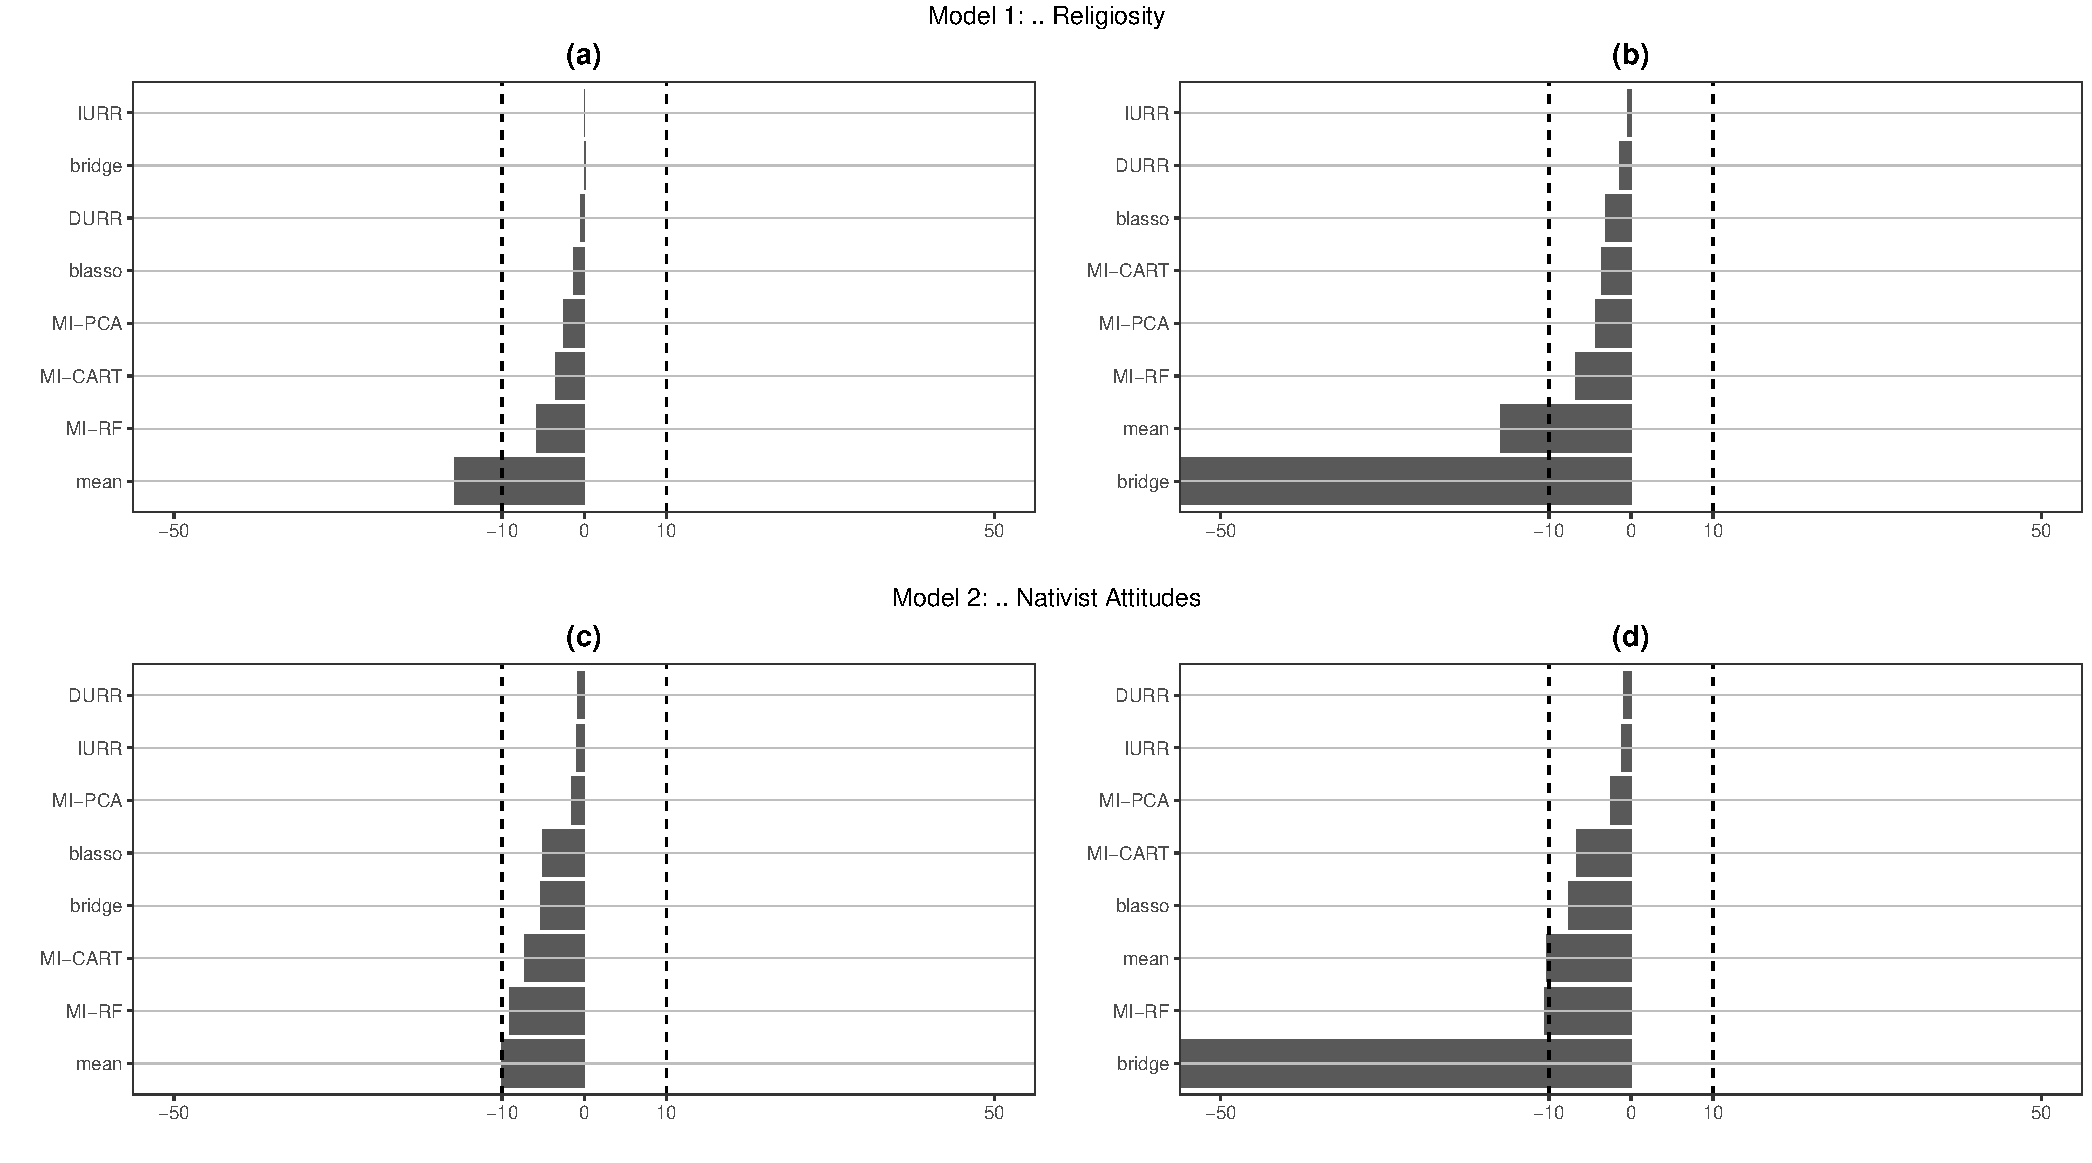
\includegraphics{\pathFIG/exp4_imp_bias.pdf}
	\caption{Bias for single parameter of interest in the two different models}
	\label{fig:exp4bias}
\end{figure}

\begin{figure}
	\centering
	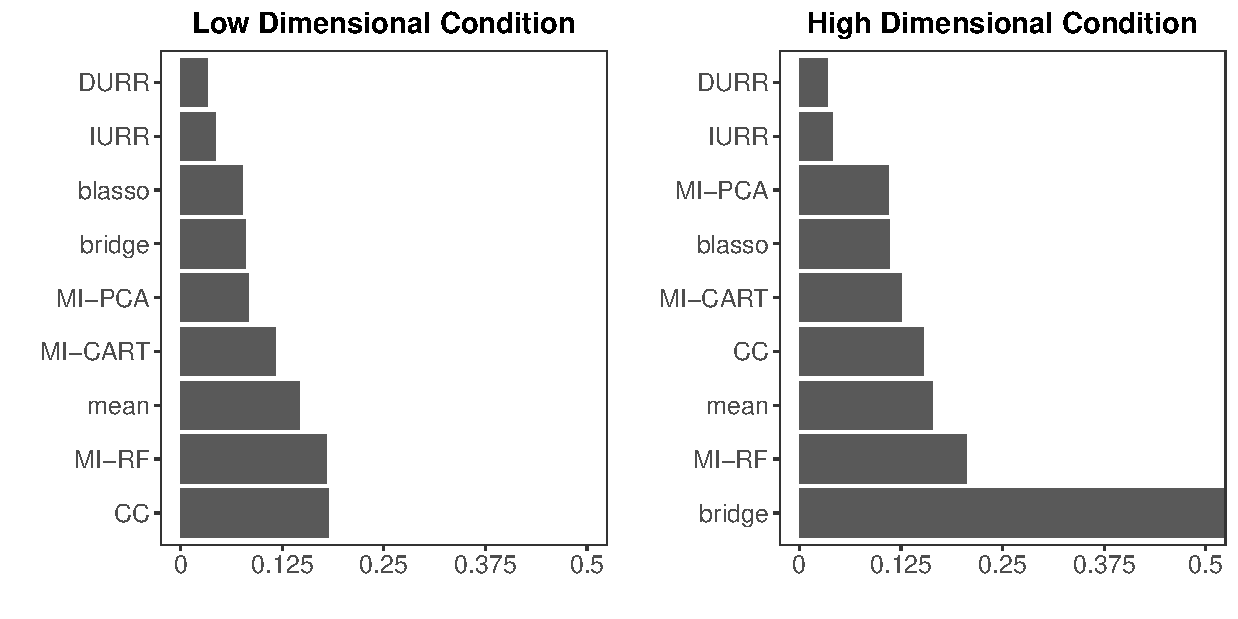
\includegraphics{\pathFIG/exp4_ed_bias.pdf}
	\caption{Euclidean distance between the vector of estimated regression coefficients and
		the vector of their true value}
	\label{fig:exp4biased}
\end{figure}

%\FloatBarrier

\subsubsection{Confidence Interval Coverage}

	\paragraph{Confidence Interval Coverage}
	Researchers interested in testing their theories based on models like the ones described will be interested
	in the confidence interval coverage of the estimates of interest.
	Figure \ref{fig:exp4ci} reports the CIC for $\beta_{1,1}$ and $\beta_{1,2}$, the focal regression coefficients 
	in the two models.

	For model \ref{eqn:lm2}, both IURR and DURR remain fairly competitive with CIC close to nominal levels, but 
	the advantage they showed in terms of bias is not carried over to this criterion.
	Both MI-PCA and Blasso provides CICs that are either equal or closer to nominal than the ones obtained with
	IURR and DURR in almost all conditions.

	For model \ref{eqn:lm1}, condition (b) shows interesting patterns: 
	\begin{itemize}
		\item all MI methods show signs of undercoverage with CIC smaller than the threshold value .93;
		\item all MI methods perform \emph{worse} than Complete Case analysis, which covers the true value 
			more frequently than with imputation (more on this below);
		\item all MI methods perform \emph{better} than the Gold Standard, which covers the true value 
			in approximately only 90\% of the replications performed.
	\end{itemize}
	
	\paragraph{Euclidean Distance}
	When looking at the more general pattern described by $d_{CIC}$, reported in \ref{fig:exp4cied}, IURR and DURR 
	return to the top of the leader-board, providing the vectors of Confidence Interval Coverages closest to 
	nominal levels.
	Furthermore, they are the only methods providing coverage equivalent to the Gold Standard method in all conditions
	for both models.

	\paragraph{Confidence Interval Width}
	The seemingly competitive coverage showed by CC in figure \ref{fig:exp4cied} is achieved with much wider 
	95\% Confidence Intervals than all other methods. 
	Figure \ref{fig:exp4ciw} shows the average Confidence Interval Width across model parameters.
	Apart from bridge in the high-dimensional conditions, CC is always showing the widest confidence intervals.
	This is of course due to the lower number of data observations used to obtained estimates, and it makes clear
	how the close to nominal coverage showed by CC in figure \ref{fig:exp4cied} is an artifice of the wider 
	confidence intervals.

	By a similar logic, we note that the less ideal behaviour of MI-PCA showed in figure \ref{fig:exp4cied} compared 
	to IURR, is not due to wider or narrower confidence intervals.
	The difference is more likely due to the larger bias that MI-PCA tends to produce (see figure 
	\ref{fig:exp4biased}).

\begin{figure}
	\centering
	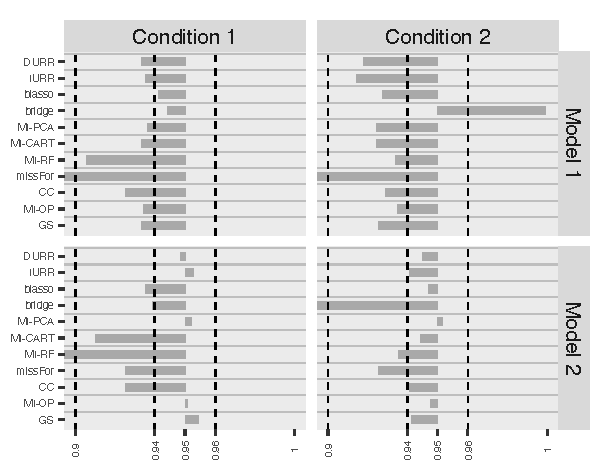
\includegraphics{\pathFIG/exp4_imp_ci.pdf}
	\caption{Confidence Interval Coverage for single parameter of interest in the two 
		different models}
	\label{fig:exp4ci}
\end{figure}

\begin{figure}
	\centering
	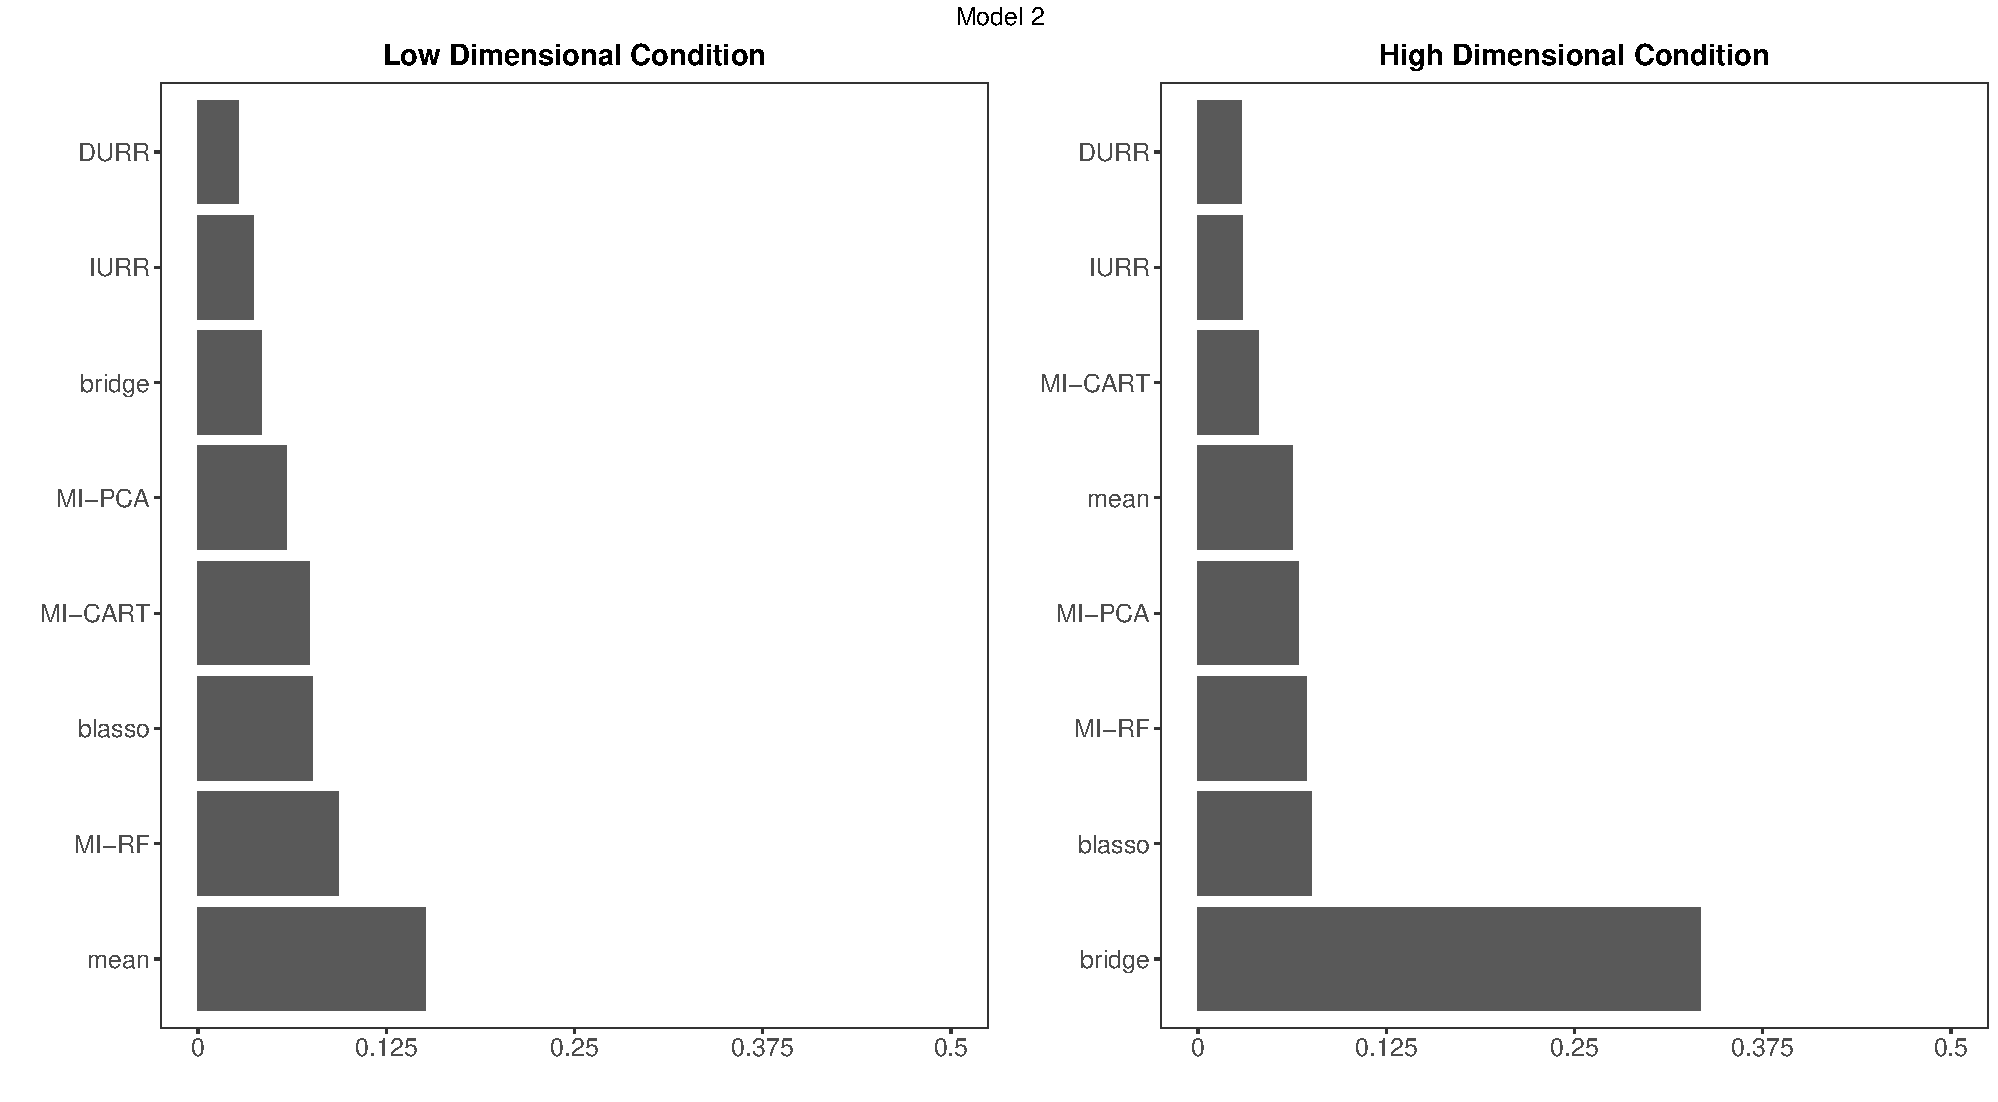
\includegraphics{\pathFIG/exp4_ed_ci.pdf}
	\caption{Euclidean distance between the vector of confidence coverages and the vector of 
		nominal coverage}
	\label{fig:exp4cied}
\end{figure}

\begin{figure}
	\centering
	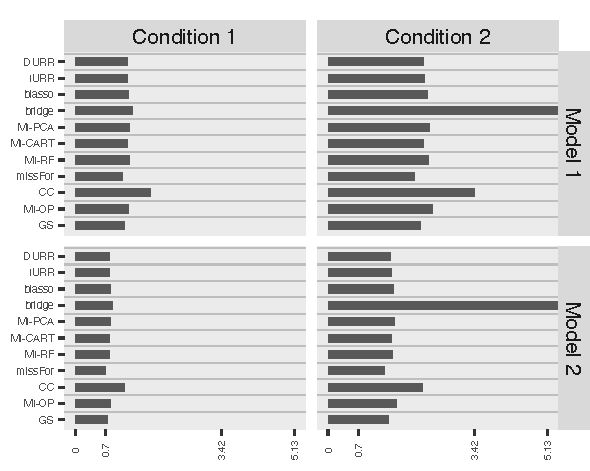
\includegraphics{\pathFIG/exp4_imp_ciw.pdf}
	\caption{Average Model Parameter Confidence Interval Width}
	\label{fig:exp4ciw}
\end{figure}

%\FloatBarrier

\subsubsection{Imputation Time}

	Figure \ref{fig:exp4time} shows the average imputation time across the different methods.
	IURR and DURR are the most time consuming methods with imputation times above the hour, 
	in our low dimensional conditions, versus imputation times of a minute or less for MI-PCA and 
	Blasso imputation.
	In the high dimensional condition, IURR and DURR are not as time-intensive, but still 
	require more then ten times the time of MI-PCA and blasso imputation.

\begin{figure}
	\centering
	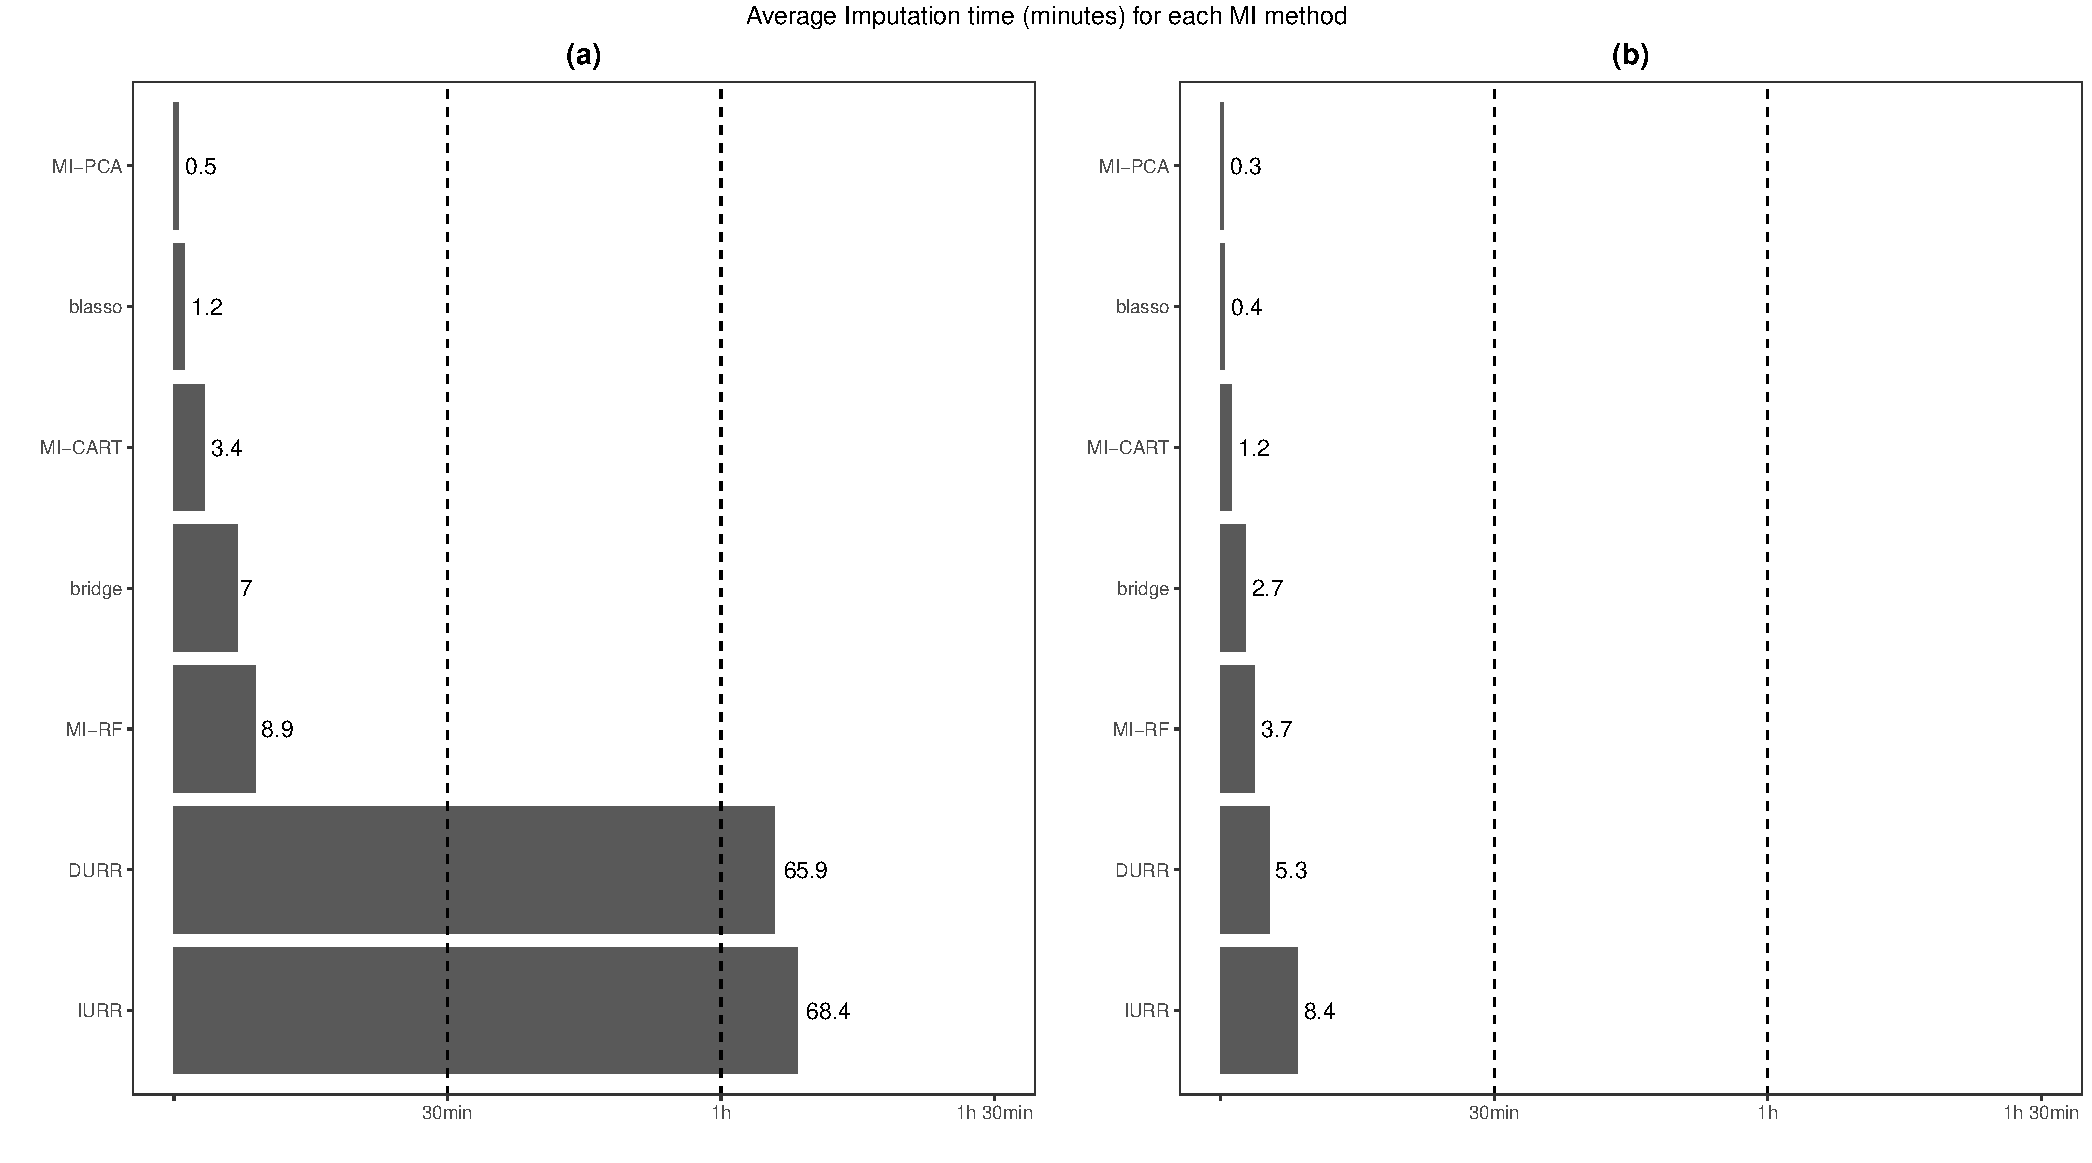
\includegraphics{\pathFIG/exp4_time.pdf}
	\caption{Average imputation time for each method}
	\label{fig:exp4time}
\end{figure}

\FloatBarrier


